\documentclass[conference]{IEEEtran}
\IEEEoverridecommandlockouts
\usepackage{cite}
\usepackage{amsmath,amssymb,amsfonts}
\usepackage{graphicx}
\usepackage{textcomp}
\usepackage{hyperref}
\usepackage{booktabs}
\def\BibTeX{{\rm B\kern-.05em{\sc i\kern-.025em b}\kern-.08em
    T\kern-.1667em\lower.7ex\hbox{E}\kern-.125emX}}
\renewcommand{\rmdefault}{cmr}
\renewcommand{\sfdefault}{cmss}
\renewcommand{\ttdefault}{cmtt}

\begin{document}

\title{Controllable Chord Progression Reharmonization via RVAE-LSTM using Perceptually-Grounded Complexity Score\\}

\author{
\IEEEauthorblockN{1\textsuperscript{st} Jos\'e Pinto-Mu\~noz}
\IEEEauthorblockA{
\textit{Departamento de Inform\'atica} \\
\textit{Universidad T\'ecnica Federico Santa Mar\'ia} \\
Santiago, Chile \\
\href{mailto:jose.pintom@usm.cl}{jose.pintom@usm.cl}}
\and
\IEEEauthorblockN{2\textsuperscript{nd} Nicol\'as Rojas-Morales}
\IEEEauthorblockA{
\textit{Departamento de Inform\'atica} \\
\textit{Universidad T\'ecnica Federico Santa Mar\'ia} \\
Valpara\'iso, Chile \\
\href{mailto:nicolas.rojasm@usm.cl}{nicolas.rojasm@usm.cl}}
}

\maketitle

\begin{abstract}
Chord progression reharmonization enriches simple harmonic sequences with greater structural complexity. Although recent generative models enable harmonic transformations while preserving tonal coherence, explicit parametric control over the level of generated harmonic complexity remains an open challenge. In this work, we propose PEARL (Perceptual Enrichment via Anchored Regularized Latent-space), an RVAE-LSTM architecture for controllable harmonic enrichment. To regulate this process, we introduce the \textbf{Perceptual Complexity Score} (PCS), a metric capturing four interpretable dimensions of harmonic complexity derived from jSymbolic features. The architecture employs a 48-dimensional binary chord encoding, a bidirectional LSTM encoder with autoregressive decoder, and auxiliary predictors that reconstruct complexity and tonal center from the latent vector. During inference, gradient ascent on the latent space controls complexity, regularized to preserve structure and tonality. Two PCS variants are proposed: a perceptually-weighted formulation and an equal-weight baseline. Results on 877k progressions show PEARL achieves 88\% tonal scale adherence, surpassing CVAE (84\%) and RVAE (76\%) baseline architectures while enabling interpretable per-dimension complexity control.
\end{abstract}

\begin{IEEEkeywords}
symbolic music generation, regressor-based VAE, harmonic complexity, chord progression enrichment, perceptual score, gradient ascent
\end{IEEEkeywords}

\section{Introduction}
Chord progressions drive the harmonic narrative of music by creating cycles of tension and release. Expanding simple harmonic sequences into richer variants is a core practice in composition, arrangement, and music education. Large-scale analyses (e.g., the McGill Billboard corpus~\cite{burgoyne2011}) reveal Western popular music relies on a narrow repertoire of triads and repeating cadential formulas. This motivates automated enrichment: transforming simple progressions into denser variants through extensions, substitutions, and reharmonizations while preserving tonal identity~\cite{cecchetti2022hearing}. Such tools already appear in digital audio workstations (DAWs) like FL Studio~\cite{flstudio_manual} and Ableton Live~\cite{ableton_expressive_chords}. Yet current symbolic generation methods lack a perceptually-grounded complexity measure and explicit control over enrichment magnitude and direction.

This work introduces PEARL (Perceptual Enrichment via Anchored Regularized Latent-space), an RVAE-based framework for controllable chord progression enrichment. At its core is the \textbf{Perceptual Complexity Score} (PCS), a four-dimensional metric from a paired-comparison listening study (N=43) that distills 11 jSymbolic features into four perceptually-meaningful dimensions (see Section~\ref{sec:pcs}). PEARL encodes progressions into a structured latent space and decodes enriched versions autoregressively. To control harmonic complexity, we perform gradient ascent on the latent vector $\mathbf{z}$, guided by an auxiliary predictor trained to estimate PCS from $\mathbf{z}$, regularized to anchor the optimized code to the original progression. We propose perceptually-weighted (PEARL-v1) and equal-weight (PEARL-v2) PCS variants. The main contributions are: (a) a perceptually-validated PCS grounded in human evaluation, (b) an RVAE-LSTM with gradient-based latent enrichment enabling per-dimension control, and (c) evaluation against CVAE and RVAE baselines~\cite{comanducci2023vae} across tonal coherence, latent space organization, and five complexity levels.

\section{Related Work}
\label{sec:relatedwork}

Symbolic music generation has evolved from sequence prediction toward controllable enrichment. Early LSTMs captured temporal structure in chord and note sequences~\cite{eck2002first,oore2020time2}, with teacher forcing ensuring stable training~\cite{williams1989learning}. Later models introduced conditioning on style, harmonic function, or key~\cite{roberts2017musicvae,herremans2017functional}, shifting from generation to controlled transformation. A recent survey~\cite{Ji2023} documents this trend toward conditional and variational methods for chord progression enrichment.

VAEs brought structured latent spaces to harmonic modeling. Uemura et al. proposed chord morphing through latent interpolation in a piano-roll VAE~\cite{uemura2018preliminary}, extended with LSTM-VAE temporal dynamics and melodic conditioning~\cite{uemura2020morphing}, and further refined with consonance-based losses and style vectors~\cite{uemura2022morphing}. Hierarchically, MusicVAE~\cite{roberts2017musicvae} organized latent spaces across temporal scales using a hierarchical decoder; MorpheuS~\cite{herremans2017functional} modeled long-range structure via tonal tension and repetition. Zhao et al.~\cite{zhao2019variational} introduced regression-based VAE conditioning for continuous latent control.

Harmonic complexity has been defined through tonal deviation, chord diversity, and unpredictability~\cite{rohrmeier2012comparing,temperley2004cognition}, with computational models quantifying perceived complexity~\cite{digiorgi2017modeling}. Comanducci et al.~\cite{comanducci2023vae} developed a perceptual complexity model using CVAEs and RVAEs, characterizing complexity by harmonic evolution, dissonance, and rhythmic density. Their approach has three notable constraints: (i) the chord vocabulary is limited to four types (maj, min, 5, 7) as 12-dimensional multi-hot vectors, omitting extensions, alterations, and bass inversions; (ii) the dataset contains only 6,311 synthetic five-chord progressions anchored to C major/minor, precluding generalization to other keys and lengths; and (iii) complexity is a scalar from a compound language model combining Prediction by Partial Matching (PPM), Hidden Markov Models (HMM), and Recurrent Neural Networks (RNN), yielding no interpretable decomposition of the contributing factors. Listening tests confirmed a correlation between conditioning values and perceived complexity, motivating our multi-dimensional metric.

\section{Our Proposal: PEARL}
\label{sec:proposal}

\begin{figure*}[t]
\centering
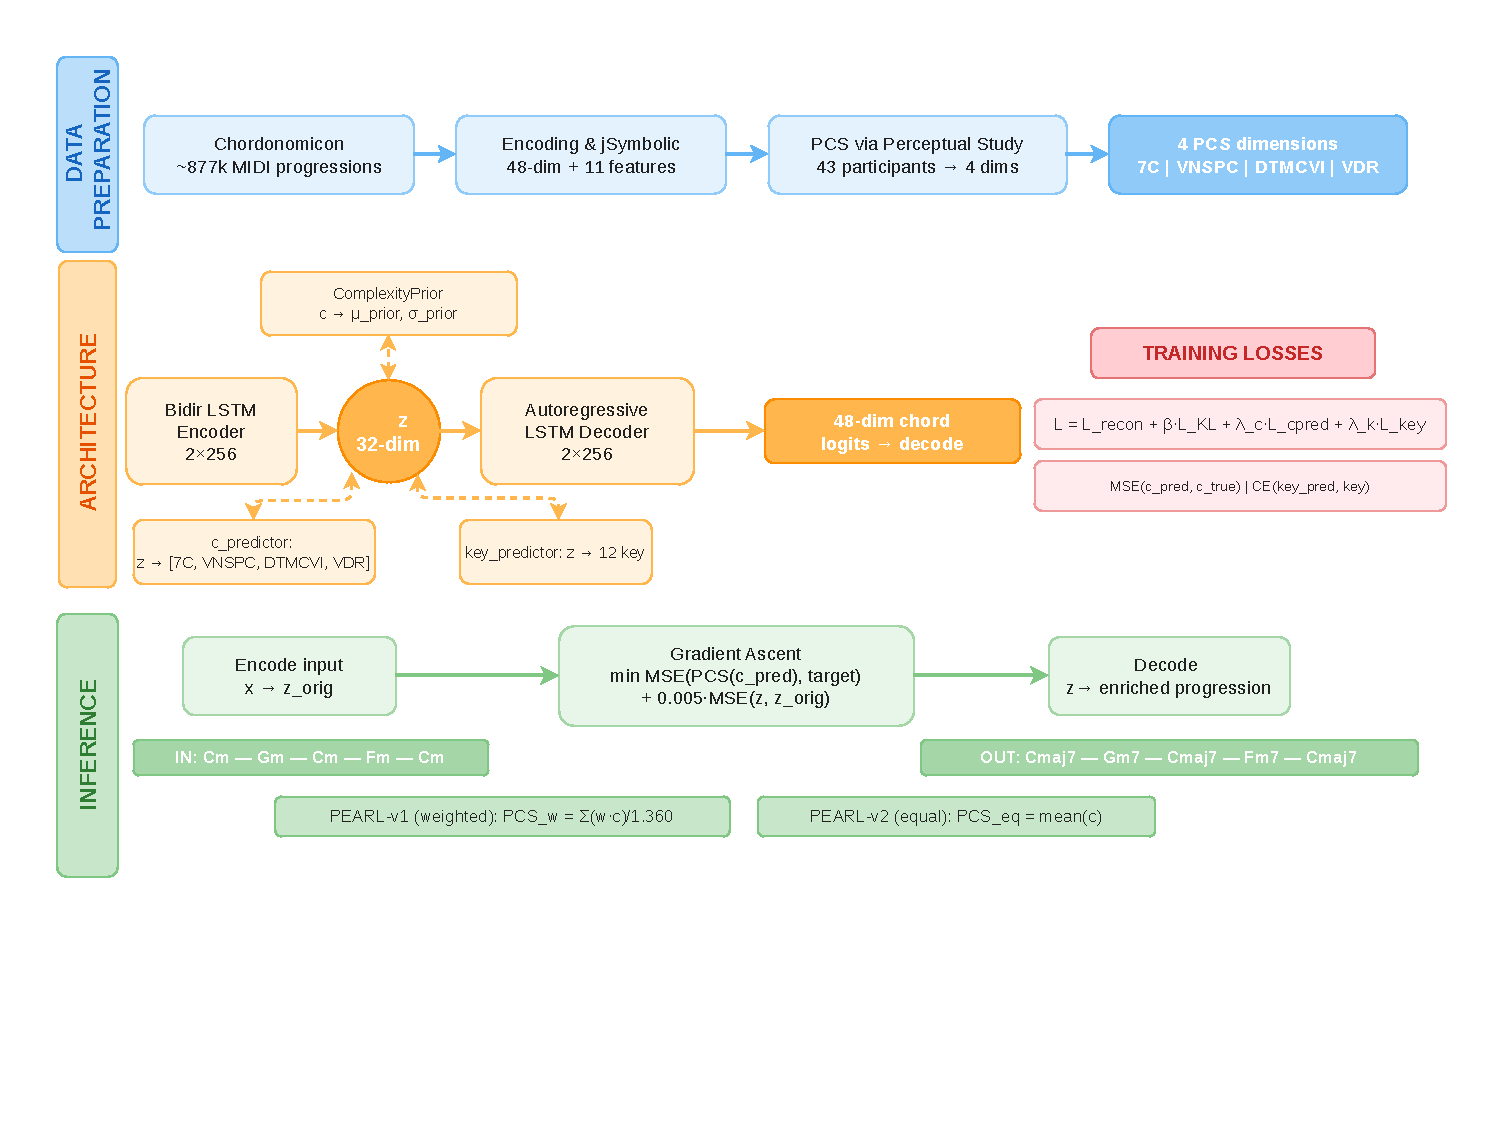
\includegraphics[width=1\textwidth, trim=0 35mm 0 5mm, clip]{img/fig2.pdf}
\caption{Overview of the PEARL pipeline. \textbf{Data Preparation} (left): chord progressions from the Chordonomicon dataset are encoded as 48-dimensional binary vectors, analyzed with jSymbolic, and labeled with the four PCS dimensions derived from the perceptual study. \textbf{Architecture} (center): an RVAE-LSTM with bidirectional encoder, autoregressive decoder, \texttt{c\_predictor} and \texttt{key\_predictor} auxiliary heads, and a conditional ComplexityPrior. \textbf{Inference \& Training} (right): gradient ascent on $\mathbf{z}$ guided by the \texttt{c\_predictor} enriches any input progression to a target PCS; training combines reconstruction, KL, and auxiliary prediction losses.}
\label{fig:pipeline}
\end{figure*}

PEARL is an RVAE architecture that conditions on a four-dimensional Perceptual Complexity Score (7C, VNSPC, DTMCVI, VDR; see Section~\ref{sec:pcs}) and enriches progressions via gradient ascent on the latent space. Figure~\ref{fig:pipeline} illustrates the pipeline: data preparation, architecture, and inference.

\subsection{Chord Encoding and Data Preparation}

Each chord is a 48-dimensional binary vector divided into seven interpretable slots. Unlike piano-roll or multi-hot encodings that treat chord tones as independent, this factored representation separates orthogonal musical attributes, allowing the model to learn valid chord structures more efficiently:

\begin{itemize}
    \item \textbf{Root} (12 dims): one-hot encoding of the root pitch class (C--B).
    \item \textbf{Quality} (8 dims): maj, min, dim, aug, sus2, sus4, no3d, other.
    \item \textbf{Seventh} (5 dims): none, dom7, maj7, dim7, aug7.
    \item \textbf{Extensions} (3 dims): multilabel flags for 9, 11, 13.
    \item \textbf{Alterations} (4 dims): multilabel flags for b9, \#9, \#11, b13.
    \item \textbf{Added notes} (3 dims): multilabel flags for add9, add11, add13.
    \item \textbf{Bass} (13 dims): one-hot for bass note (C--B + root/no-slash).
\end{itemize}

This 48-dimensional representation is fully interpretable: each sub-vector can be decoded back to a human-readable chord symbol via deterministic argmax and threshold operations. The seven-slot design separates independent musical attributes, allowing the model to learn compositional rules (e.g., which extensions co-occur with which seventh types) directly from the data. A progression of $T$ chords is encoded as a matrix $\mathbf{X} \in \{0,1\}^{T \times 48}$.

\subsection{Perceptual Complexity Score (PCS)}
\label{sec:pcs}

In this work, harmonic complexity is defined as the degree to which chord changes in a progression are varied, rich, and unexpected, encompassing harmonic rhythm, dissonance within chords, and tonal evolution~\cite{rohrmeier2012comparing,temperley2004cognition}. To ground this concept in measurable, perceptually-relevant features, we conducted a paired-comparison listening study---a well-established psychophysical method for ranking stimuli when absolute ratings are unreliable across participants. In this design, each participant evaluates pairs rather than assigning absolute scores, producing relative judgments that are more stable across subjects with different internal reference frames. A total of 53 participants completed the test. Two control pairs with clearly different complexity levels were included to verify understanding and detect inattentive responses; participants who responded inconsistently to both control questions were excluded, retaining 43 valid participants. Participants completed a questionnaire derived from the Goldsmiths Musical Sophistication Index (GMSI)~\cite{mullensiefen2014musicality} (Musical Training Score $MTS = \sum_{i=1}^{n} s_i/52$) and were stratified into three Musical Sophistication Index (MSI) levels: Low, Medium, and High.

Participants compared pairs of audio excerpts without being informed of their origin and selected the more complex progression on a five-point scale (\textit{A much more complex than B}, \textit{A more complex than B}, \textit{both equally complex}, \textit{B more complex than A}, \textit{B much more complex than A}). In total, 1032 paired observations were collected across all MSI levels. Each of the 11 jSymbolic features was correlated against the human complexity ratings within each MSI level. A feature was retained if it satisfied two criteria: (1) statistical significance ($p < 0.05$) in at least one MSI level (i.e., a non-null signal), and (2) the correlation must have the same sign across all MSI levels where it reached statistical significance. This two-stage procedure---null-signal screening followed by sign-consistency verification---ensures reproducible feature selection across heterogeneous subpopulations by discarding both irrelevant and contradictory predictors~\cite{zhao2025reproducible}.

Four of 11 features satisfied both criteria (Table~\ref{tab:pcs_selection}). Using the absolute correlation avoids penalizing features with strong negative associations to complexity (e.g., features that decrease as human-rated complexity increases). Each retained feature's weight $w_d$ is computed as the mean of absolute correlations across the three MSI levels: $w_d = (|r_{\text{High}}| + |r_{\text{Low}}| + |r_{\text{Medium}}|) / 3$. The PCS is defined as a weighted sum of min-max normalized feature values (normalized across the entire training dataset so that the maximum possible value maps to 1.0), clipped to $[0, 1]$:

\begin{equation}
\begin{split}
PCS_w = \bigl(&0.443 \cdot \text{7C} + 0.378 \cdot \text{VNSPC} \\
              + &0.338 \cdot \text{DTMCVI} + 0.201 \cdot \text{VDR}\bigr) \;/\; 1.360
\end{split}
\label{eq:pcs_weighted}
\end{equation}

\begin{table}[h]
\centering
\caption{Correlation ($r$) and $p$-values of jSymbolic features with perceived complexity. Bold = $p < 0.05$. $\checkmark$ = retained.}
\label{tab:pcs_selection}
\resizebox{\columnwidth}{!}{
\begin{tabular}{lrrrrrrr}
\toprule
\textbf{Feature} & \textbf{$r$ (High)} & \textbf{$r$ (Low)} & \textbf{$r$ (Medium)} & \textbf{$p$ (High)} & \textbf{$p$ (Low)} & \textbf{$p$ (Medium)} & \textbf{Retained} \\
\midrule
7C (Seventh Chords)      & 0.580 & 0.239 & 0.510 & \textbf{0.003} & 0.261 & \textbf{0.011} & $\checkmark$ \\
VNSPC (Var. Sim. PCs)    & 0.475 & 0.174 & 0.484 & \textbf{0.019} & 0.416 & \textbf{0.017} & $\checkmark$ \\
DTMCVI (Dist. MCVI)      & 0.325 & 0.209 & 0.481 & 0.121 & 0.327 & \textbf{0.017} & $\checkmark$ \\
VDR (Vert. Diss. Ratio)  & -0.125 & 0.406 & 0.071 & 0.559 & \textbf{0.049} & 0.743 & $\checkmark$ \\
\midrule
CC (Complex Chords)       & -0.363 & 0.356 & -0.158 & 0.081 & 0.088 & 0.460 & --- \\
NSC (Non-Standard Chords) & -0.189 & 0.240 & -0.011 & 0.375 & 0.259 & 0.958 & --- \\
ST (Standard Triads)      & -0.213 & -0.382 & -0.331 & 0.318 & 0.065 & 0.114 & --- \\
VS (Vertical Sevenths)    & -0.258 & 0.313 & -0.115 & 0.223 & 0.136 & 0.593 & --- \\
VMS (Vert. Minor Sec.)    & 0.107 & 0.271 & 0.201 & 0.618 & 0.200 & 0.347 & --- \\
VT (Vertical Tritones)    & -0.119 & 0.034 & -0.109 & 0.581 & 0.873 & 0.611 & --- \\
PRTMCVI (Prev. Ratio)     & -0.114 & 0.079 & -0.072 & 0.596 & 0.712 & 0.738 & --- \\
\bottomrule
\end{tabular}
}
\end{table}



The sum of weights (1.360) acts as a normalization constant. This gives nearly twice as much weight to Seventh Chords (0.443) as to Vertical Dissonance Ratio (0.201), reflecting the stronger and more consistent correlation of 7C with perceived complexity across expertise levels---particularly at the High MSI level ($r{=}0.580$, $p{=}0.003$). Musically, 7C captures the frequency of seventh chords, VNSPC measures variability in simultaneous pitch-class density, DTMCVI quantifies how far apart the two most common vertical intervals are, and VDR represents the proportion of dissonant vertical intervals.

We additionally define an equal-weight variant for comparison:

\begin{equation}
PCS_{eq} = \frac{7C + VNSPC + DTMCVI + VDR}{4}
\label{eq:pcs_equal}
\end{equation}

We refer to the model using Equation~\ref{eq:pcs_weighted} as \textbf{PEARL-v1 (weighted)} and the model using Equation~\ref{eq:pcs_equal} as \textbf{PEARL-v2 (equal)}. V1 prioritizes seventh chords via the perceptual weights, aligning enrichment with how human listeners perceive complexity; v2 distributes effort uniformly, providing a reference that isolates the effect of the weighting scheme from other architectural choices.

\subsection{Model Architecture}

The model is an RVAE with bidirectional LSTM encoder and autoregressive LSTM decoder. In the RVAE~\cite{comanducci2023vae,zhao2019variational}, a regressor network estimates the conditioning variable from the latent code, and a conditional prior $p(\mathbf{z}|\mathbf{c})$ is learned jointly---unlike CVAEs that simply concatenate $\mathbf{c}$ to the encoder input.

\textbf{Encoder.} The encoder is a 2-layer bidirectional LSTM with hidden size 256. Bidirectionality allows each chord to be encoded with context from both past and future positions, which is critical for representing harmonic function (e.g., distinguishing a dominant chord that resolves from one that does not). Given an input chord sequence $\mathbf{X} \in \{0,1\}^{T \times 48}$, the final hidden states from both directions are concatenated and projected via two linear layers to produce the posterior parameters $\boldsymbol{\mu}, \log\boldsymbol{\sigma}^2 \in \mathbb{R}^{d_z}$. A latent vector is sampled via the reparameterization trick:

\begin{equation}
\mathbf{z} = \boldsymbol{\mu} + \boldsymbol{\sigma} \odot \boldsymbol{\epsilon}, \quad \boldsymbol{\epsilon} \sim \mathcal{N}(0, \mathbf{I})
\label{eq:reparam}
\end{equation}

\textbf{ComplexityPrior.} A conditional prior $p(\mathbf{z}|\mathbf{c})$ is learned via a small MLP that maps the 4 PCS dimensions to prior parameters $\boldsymbol{\mu}_{\text{prior}}, \log\boldsymbol{\sigma}^2_{\text{prior}} \in \mathbb{R}^{d_z}$, enabling sampling at a desired complexity without real input.

\textbf{Decoder.} The decoder is a 2-layer autoregressive LSTM with hidden size 256. At each time step $t$, the latent vector $\mathbf{z}$ is concatenated with the previous output chord and fed to the LSTM. A linear head projects the LSTM output to 48 logits. With $z\_only\_decoder{=}\text{True}$, the decoder receives $\mathbf{z}$ directly rather than the condition vector $\mathbf{c}$---this design isolates complexity control to the latent space, ensuring that varying $\mathbf{c}$ at inference time has no effect on the output and that enrichment must be accomplished by \textit{moving} $\mathbf{z}$.

\textbf{CPredictor.} A 2-hidden-layer MLP (64 units, ReLU) maps $\mathbf{z}$ to predicted PCS values $\hat{\mathbf{c}} = (\hat{7C}, \hat{VNSPC}, \hat{DTMCVI}, \hat{VDR}) \in \mathbb{R}^4$. Its gradient $\partial \hat{c}_d / \partial \mathbf{z}$ tells us in which direction to move $\mathbf{z}$ to increase a specific complexity dimension $d$, enabling the gradient-based enrichment described in Section III-D.

\textbf{KeyPredictor.} An analogous MLP maps $\mathbf{z}$ to 12-class key logits, training $\mathbf{z}$ to encode tonal center information. This auxiliary loss shapes the latent space so that $\mathbf{z}$ carries key information, which---combined with the regularization in Section III-D---indirectly helps preserve tonality during enrichment. The predicted key is also used post-hoc to verify tonal coherence in the generated progressions.

\subsection{Inference: Gradient Ascent on $\mathbf{z}$}
\label{sec:grad_ascent}

The core novelty of PEARL is the inference procedure: rather than sampling multiple candidates and filtering them, we directly optimize $\mathbf{z}$ to reach a user-specified PCS target. This gradient-based approach is deterministic given the same initialization and target, providing reproducibility and fine-grained control that would be impractical with random sampling. Given an input progression encoded as $\mathbf{z}_{\text{orig}}$, we solve:

\begin{equation}
\begin{split}
\mathbf{z}^* = \arg\min_{\mathbf{z}} \Bigl[ &\text{MSE}\bigl(PCS(\texttt{c\_pred}(\mathbf{z})),\; t\bigr) \\
                                           + &\lambda_{\text{reg}} \cdot \text{MSE}(\mathbf{z}, \mathbf{z}_{\text{orig}}) \Bigr]
\end{split}
\label{eq:grad_ascent}
\end{equation}

using Adam optimization (lr = 0.5, 90 steps, gradient clipping at 1.0) with $\lambda_{\text{reg}} = 0.005$. The first term drives the predicted PCS toward the target; the second term anchors $\mathbf{z}$ to its original location, preserving the progression's tonal context while allowing substantial chord-level variation. Once optimized, $\mathbf{z}^*$ is fed to the autoregressive decoder to generate the enriched chord sequence.

The gradient through the \texttt{c\_predictor} reflects the PCS variant used: v1's gradient is proportional to the perceptual weights, while v2 distributes uniformly (see Section~\ref{sec:pcs}). Individual dimensions can also be targeted by setting the loss to $\text{MSE}(\hat{c}_d, target_d)$ for a specific dimension $d$.

\section{Experimental Setup}

This section describes the training configuration, dataset, baselines, and evaluation protocols used to assess PEARL's enrichment capabilities.\footnote{The complete code, trained model checkpoint, experiment results (audio + MIDI), survey data, and experiment scripts are available at \url{https://github.com/Pepebeats-flp/pearl-sc}.}

\subsection{Training Configuration}

Table~\ref{tab:hyperparams} lists the hyperparameters used for training. The model was trained for 30 epochs on approximately 877k progressions from the Chordonomicon dataset~\cite{kantarelis2024chordonomicon}.

\begin{table}[h]
\centering
\caption{Training hyperparameters.}
\label{tab:hyperparams}
\resizebox{\columnwidth}{!}{
\begin{tabular}{ll}
\toprule
\textbf{Parameter} & \textbf{Value} \\
\midrule
Chord dimension ($d_{\text{chord}}$) & 48 \\
Encoder LSTM hidden dim & 256 \\
Encoder LSTM layers & 2 (bidirectional) \\
Decoder LSTM hidden dim & 256 \\
Decoder LSTM layers & 2 \\
Latent dimension ($d_z$) & 32 \\
Condition dimension ($d_c$) & 16 (4 PCS + 12 key) \\
Dropout & 0.2 \\
Word dropout & 0.7 (70\% of inputs zeroed) \\
Optimizer & Adam, lr = $5\times10^{-4}$ \\
Batch size & 256 \\
Gradient clipping & 5.0 \\
$\beta$ (KL weight) & 0.01 \\
Free bits (total / per-dim) & 1.0 / 0.25 \\
KL cycle & 10 epochs \\
Scheduled sampling & 1.0 $\rightarrow$ 0.3 (15 epochs) \\
\bottomrule
\end{tabular}
}
\end{table}

The total loss function combines VAE terms with auxiliary prediction losses:

\begin{equation}
\mathcal{L} = \mathcal{L}_{\text{recon}} + \beta \cdot \mathcal{L}_{\text{KL}} + \lambda_c \cdot \mathcal{L}_{\text{c\_pred}} + \lambda_k \cdot \mathcal{L}_{\text{key\_pred}}
\label{eq:total_loss}
\end{equation}

where $\mathcal{L}_{\text{recon}}$ is binary cross-entropy (BCE) with length masking; $\mathcal{L}_{\text{KL}}$ uses per-dimension free bits (0.25) and total free bits (1.0) to prevent posterior collapse; $\mathcal{L}_{\text{c\_pred}} = \text{MSE}(\hat{\mathbf{c}}, \mathbf{c}_{\text{true}})$; and $\mathcal{L}_{\text{key\_pred}}$ is cross-entropy over 12 key classes. We set $\lambda_c = 10.0$ (scaling MSE to BCE magnitude) and $\lambda_k = 0.5$ (weak auxiliary signal). The cyclic KL schedule raises $\beta$ from 0 to $\beta_{\text{target}} = 0.01$ over 10 epochs and resets periodically to prevent KL collapse. Teacher forcing decays from 1.0 to 0.3 over 15 epochs; word dropout zeros 70\% of input tokens to prevent the decoder from ignoring $\mathbf{z}$. Training converged after 30 epochs (val loss 4.24, KL $\approx 6$--$7$ nats, all 32 latent dimensions active). The bypass delta (increase in BCE when zeroing $\mathbf{z}$ at teacher forcing 0; a large delta confirms the decoder cannot reconstruct without $\mathbf{z}$) was 2.77 BCE, confirming decoder reliance on $\mathbf{z}$ and meaningful use of all dimensions. An 80/10/10 stratified split was used, ensuring that progressions from the same song do not appear in both training and test sets; all Section~V results are computed on the held-out test set.

\subsection{Dataset and Baselines}

The training dataset uses Chordonomicon~\cite{kantarelis2024chordonomicon}, which provides chord progressions for approximately 666k songs parsed from user-contributed guitar tablatures. Following the procedure in~\cite{kantarelis2024chordonomicon}, structural sections are treated as independent progressions, expanding the dataset to approximately 877k progressions, processed with jSymbolic~2.2~\cite{mckay2018jsymbolic} for PCS labeling.

Following~\cite{comanducci2023vae}, we evaluate on \textit{Cmin -- Gmaj -- Cmin -- Fmin -- Cmin} (5 chords, C minor tonality) against CVAE and RVAE baselines at five complexity levels (class 1--5). PEARL uses five analogous PCS targets (0.00, 0.25, 0.50, 0.75, 1.00) for both v1 and v2.

\subsection{Evaluation Metrics}

We evaluate the generated progressions using standard jSymbolic~2.2 features~\cite{mckay2018jsymbolic}, following the methodology of~\cite{uemura2022morphing}, and derived metrics. The four PCS dimensions (7C, VNSPC, DTMCVI, VDR) are extracted via jSymbolic; tonal coherence is assessed with respect to the key of the input progression as defined in Western tonal theory~\cite{temperley2004cognition}. These metrics capture two complementary aspects: enrichment efficacy (how well the PCS target is reached and through which dimensions) and tonal fidelity (how well the original key and chord qualities are preserved).
\begin{itemize}
    \item \textbf{PCS achieved:} actual PCS value after enrichment vs.\ target.
    \item \textbf{Per-dimension delta ($\Delta_d$):} absolute change in each PCS dimension ($\Delta 7C$, $\Delta VNSPC$, $\Delta DTMCVI$, $\Delta VDR$).
    \item \textbf{Ratio $\Delta 7C / \Sigma\Delta_{\text{others}}$:} how much complexity increase comes from seventh chords vs.\ other dimensions.
    \item \textbf{Seventh chord ratio:} \% of chords containing a seventh.
    \item \textbf{Chord type distribution:} classification into triads, 7ths, suspended, diminished/augmented, and altered chords.
    \item \textbf{Scale adherence (Scale \%):} \% chord roots in the input key's scale.
    \item \textbf{Tonal coherence:} (i) root overlap with input, (ii) quality preservation, (iii) \texttt{key\_predictor} consistency.
    \item \textbf{Latent displacement:} Euclidean distance $\|\mathbf{z}^* - \mathbf{z}_{\text{orig}}\|$.
\end{itemize}

\section{Results}

We present results on latent space organization, generalization across keys and progression lengths, baseline comparison, gradient distribution analysis, and tonal coherence.

\subsection{Latent Space Organization}

We first analyze the structure of the trained latent space to verify that complexity and key are effectively encoded in $\mathbf{z}$. Table~\ref{tab:latent_stats} summarizes key statistics.

\begin{table}[h]
\centering
\caption{Latent space statistics.}
\label{tab:latent_stats}
\resizebox{\columnwidth}{!}{
\begin{tabular}{ll}
\toprule
\textbf{Metric} & \textbf{Value} \\
\midrule
Active dimensions ($KL > 0.01$) & 32/32 (100\%) \\
Total KL & 32.72 nats \\
Per-dim KL range & 0.12 -- 3.39 \\
Mean posterior std ($\boldsymbol{\sigma}$) & 1.13 \\
PCA variance: 2 / 5 / 10 PCs & 42.6\% / 65.3\% / 83.8\% \\
CPredictor MSE & 0.0034 \\
KeyPredictor accuracy & 98.4\% \\
\midrule
Top $|r|$ with 7C & $z_{15}$ (-0.93), $z_{26}$ (-0.88), $z_{1}$ (-0.84) \\
Top $|r|$ with VDR & $z_{26}$ (-0.86), $z_{22}$ (+0.77), $z_{30}$ (-0.75) \\
\bottomrule
\end{tabular}
}
\end{table}

All 32 latent dimensions are active, indicating no posterior collapse. The total KL of 32.72 nats reflects a well-regularized latent space. The CPredictor achieves an MSE of 0.0034, confirming that the four PCS dimensions can be accurately reconstructed from $\mathbf{z}$---a prerequisite for gradient ascent enrichment. The KeyPredictor reaches 98.4\% accuracy, confirming that $\mathbf{z}$ encodes strong tonal information learned during training; this latent organization, together with the regularization anchor, underlies PEARL's high scale adherence (88\%) despite substantial latent displacement.

\begin{figure*}[t]
\centering
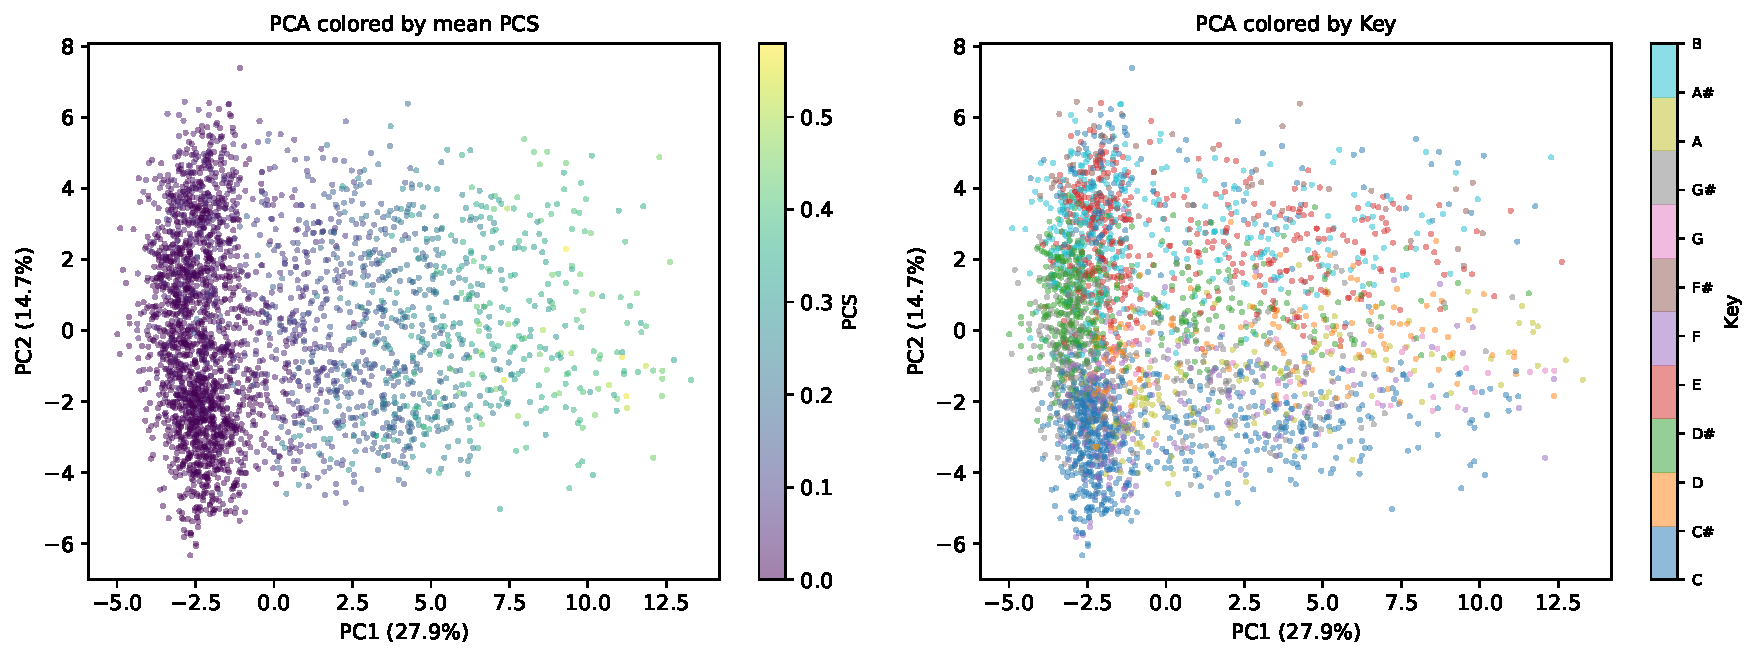
\includegraphics[width=0.95\textwidth]{img/pca_colored.pdf}
\caption{PCA projection of 3,000 encoded progressions.
Left: colored by mean PCS value (darker = higher complexity). Right: colored by detected key.
The first two PCs capture 42.6\% of latent variance, revealing a smooth complexity gradient
and clear tonal clustering.}
\label{fig:pca}
\end{figure*}

Figure~\ref{fig:pca} shows a PCA projection of 3,000 encoded progressions. The left panel reveals a smooth gradient from low to high mean PCS across the latent manifold, indicating that complexity information is structurally embedded in $\mathbf{z}$. The right panel shows clear clustering by tonal center, confirming that the \texttt{key\_predictor} loss successfully organized $\mathbf{z}$ by key during training. This dual organization---complexity as a continuous gradient, key as discrete clusters---reflects the multi-task objective where $\mathbf{z}$ must simultaneously support chord reconstruction, complexity regression, and key classification.

Per-dimension correlation analysis further supports this pattern: $z_{15}$ and $z_{26}$ correlate at $r = -0.93$ and $r = -0.88$ with 7C, while $z_{26}$ also correlates at $r = -0.86$ with VDR, acting as a broadly-tuned dissonance dimension. Dimension $z_{22}$ is positively tuned to VDR ($r = +0.77$). This strong tuning likely contributes to the reliable convergence of gradient ascent, as the \texttt{c\_predictor} can exploit these specialized latent directions. Per-dimension KL values range from 0.12 to 3.39 nats (all above the 0.01 active threshold), and z standard deviations cluster around 1.0--1.3, consistent with a unit-Gaussian prior and indicating healthy latent utilization.

\subsection{Generalization Across Keys and Progression Lengths}

Before comparing against baselines, we first verify that PEARL's enrichment generalizes beyond a single test progression by evaluating its behavior across a range of keys and progression lengths. Table~\ref{tab:key_generalization} reports results for 11 progressions in different keys (7 major, 4 minor), each enriched to PCS = 0.50 using PEARL-v1.

\begin{table}[h]
\centering
\caption{Key generalization: PEARL-v1 enrichment to PCS = 0.50 across 11 keys. Scale = \% of chord roots belonging to the key's scale.}
\label{tab:key_generalization}
\resizebox{\columnwidth}{!}{
\begin{tabular}{lccl}
\toprule
\textbf{Key} & \textbf{PCS} & \textbf{Scale \%} & \textbf{Enriched progression} \\
\midrule
C major       & 0.473 & 50\%  & C--C--D\#no3d--D\# \\
D major       & 0.485 & 75\%  & D--D--A\#--D \\
E major       & 0.475 & 75\%  & E--Eno3d--D--E \\
F major       & 0.453 & 100\% & A\#maj7--Gm7--A\#7--A\#7 \\
G major       & 0.477 & 100\% & G--Gno3d--G--G \\
A major       & 0.477 & 100\% & A--D--D--A \\
B$\flat$ major & 0.453 & 100\% & B$\flat$7--B$\flat$7--B$\flat$--B$\flat$7 \\
C minor       & 0.474 & 75\%  & E--G\#no3d7--D\#no3d--D \\
D minor       & 0.485 & 75\%  & A7--Em--E--G\# \\
E minor       & 0.473 & 75\%  & Dno3d--Eno3d--Eno3d--D\#no3d \\
A minor       & 0.476 & 50\%  & Am--C\#no3d7--C\#m--Eno3d \\
\bottomrule
\end{tabular}
}
\end{table}

PCS targets are reached across all keys (0.453--0.485), confirming robust convergence across tonalities. Key preservation (whether the \texttt{key\_predictor} correctly identifies the original key) stands at 6/11 (55\%), with average scale adherence of 80\%. Keys where preservation fails (e.g., C major, C minor, A minor) drift toward closely related keys, such as the relative major (C minor $\to$ E$\flat$ major) or parallel major (A minor $\to$ A major), while roots largely stay in-scale.

Length generalization (4--12 chords, C minor, PCS=0.50) is shown in Table~\ref{tab:length_generalization}.

\begin{table}[h]
\centering
\caption{Length generalization: PEARL-v1 enrichment to PCS = 0.50 for C minor progressions of varying lengths.}
\label{tab:length_generalization}
\resizebox{\columnwidth}{!}{
\begin{tabular}{cccc}
\toprule
\textbf{Length} & \textbf{PCS} & \textbf{Scale \%} & \textbf{Chord types observed} \\
\midrule
4  & 0.475 & 100\% & no3d \\
6  & 0.478 & 100\% & maj triad, min triad, no3d \\
8  & 0.474 & 100\% & maj7, min7, minmaj7 \\
10 & 0.477 & 100\% & min triad, no3d \\
12 & 0.476 & 100\% & maj triad, no3d \\
\bottomrule
\end{tabular}
}
\end{table}

PCS convergence and scale adherence are unaffected by progression length, with 100\% scale adherence across all tested lengths. Longer progressions exhibited richer chord types (e.g., maj7, min7, minmaj7 at length 8) not observed at shorter lengths; whether additional temporal context systematically benefits diversity warrants further investigation.

\subsection{Progression Generation Across Complexity Levels}

Table~\ref{tab:progression_comparison} shows the chord progressions generated by each model across the five complexity levels. All results are presented in a unified notation (e.g., \textit{Cmin} for C minor, \textit{Gmaj} for G major).

\begin{table*}[h!]
\centering
\caption{Generated chord progressions across five complexity levels. Input: \textit{Cmin -- Gmaj -- Cmin -- Fmin -- Cmin}.}
\label{tab:progression_comparison}
\resizebox{0.95\textwidth}{!}{
\begin{tabular}{cllll}
\toprule
\textbf{Level} & \textbf{CVAE} & \textbf{RVAE} & \textbf{PEARL-v1 (PCS\_w)} & \textbf{PEARL-v2 (PCS\_eq)} \\
\midrule
1 & Cmin Gmaj Cmin Fmin Cmin & Cmin Gmaj G\#maj G7 Cmin & Emin Cmaj Cmaj Amaj Cmaj & Dmin Cmaj D\#maj Dmin Amin \\
2 & Cmin Gmaj C7 Fmin Cmin & Cmin Gmaj Cmin G7 Cmin & G\#min Cmin Ano3d Cmaj Dmin & Cno3d Dmaj Dmin Cmin Cno3d \\
3 & Cmin Gmaj A7 Fmaj Cmin & Cmin Gmaj F\#7 B7 Cmin & Cno3d Cmaj Cno3d Cmaj7 Cno3d & Cno3d Eno3d Cno3d Cmaj Cno3d \\
4 & Cmin Gmaj F\#dim7 F7 Cmin & Cmin Gmaj F\#7 F7 Cmin & Gminmaj7 Cno3d Cno3d Cmaj Cmin7 & Cno3d Cno3d Emin Cno3d Cmin \\
5 & Cmin Emin Emin Fmaj Cmin & Cmin Emin A7 F\#7 Cmin & Gmaj Cmin Cno3dmaj7 Dno3d Dmin7 & Cno3d D\#maj Cmaj Cmin Dno3d7 \\
\bottomrule
\end{tabular}
}
\end{table*}

Figure~\ref{fig:seventh_comparison} quantifies the seventh chord counts across all four models and five complexity levels. PEARL-v1 and v2 successfully reach their PCS targets, with gradient ascent converging in approximately 20--30 steps. The CVAE and RVAE baselines use a different complexity metric; however, since both their five-level scheme and our targets represent increasing harmonic complexity, their seventh chord counts are directly comparable as a coarse indicator of enrichment intensity.

At moderate-to-high complexity levels (3--5), v1 generates maj7 and altered dominant chords, while v2 produces a more diverse mixture of suspended, diminished, and non-third chords, consistent with a more distributed enrichment strategy. The latent displacement $\|\Delta\mathbf{z}\| = \|\mathbf{z}^* - \mathbf{z}_{\text{orig}}\|$ grows monotonically with target PCS, from $\sim$0.1 at level 1 to $\sim$7 at level 5, with similar magnitudes for both variants.

\begin{figure}[t]
\centering
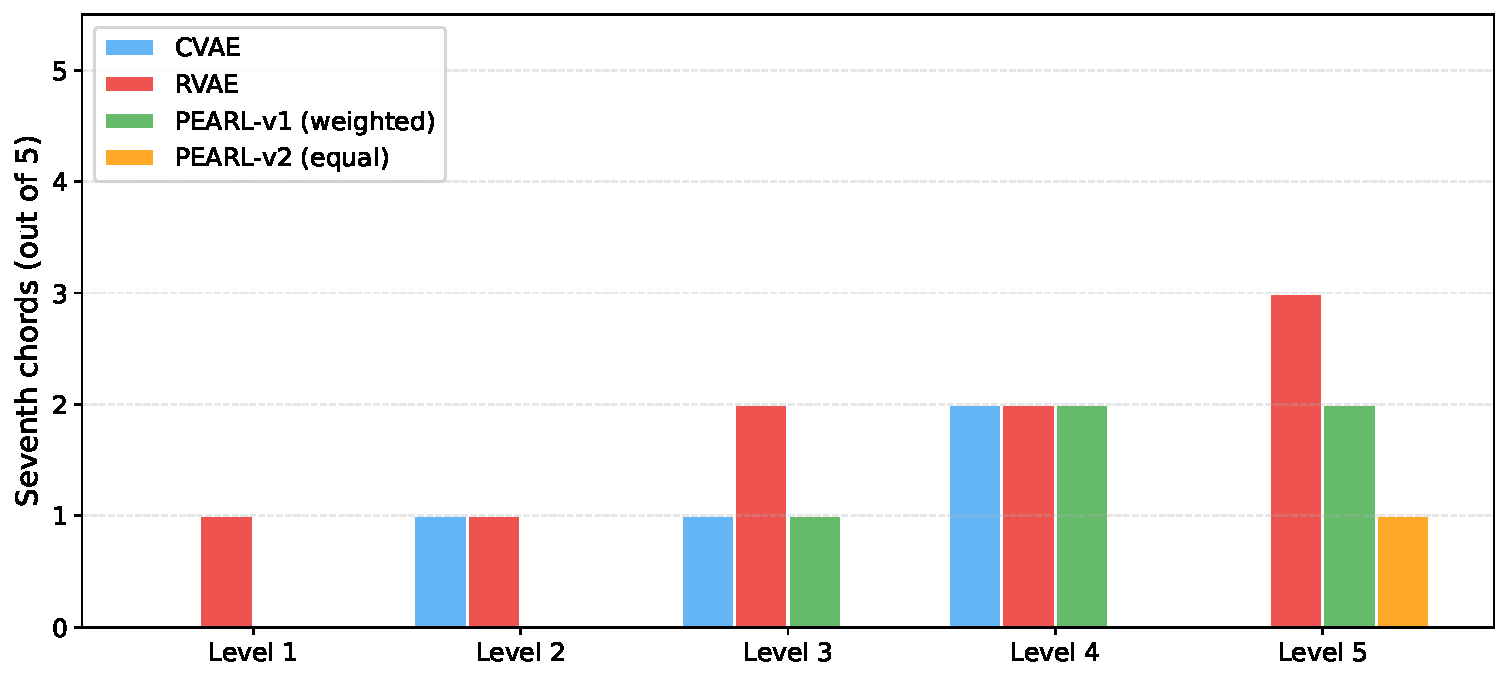
\includegraphics[width=\columnwidth]{img/seventh_comparison.pdf}
\caption{Seventh chords generated per model across five complexity levels. Input: \textit{Cmin -- Gmaj -- Cmin -- Fmin -- Cmin}.}
\label{fig:seventh_comparison}
\end{figure}

\subsection{Gradient Distribution and Comparison with Baselines}

The ratio $\Delta 7C / \Sigma\Delta_{\text{others}}$ reveals the fundamental difference between the two PEARL variants by quantifying how much of the complexity gain is driven specifically by seventh chords versus the other three dimensions. At low target levels (0.00--0.25), both variants show near-zero ratios. At higher targets, v1 consistently exhibits larger ratios than v2: at target 0.75, v1 directs 14\% of the total dimension change through 7C (vs.\ 6\% for v2); at target 1.00, v1 reaches 20\% (vs.\ 12\% for v2). This reflects the perceptual weights: v1's 0.443 weight on 7C produces a stronger gradient toward seventh-chord-rich latent regions.

The CVAE and RVAE baselines lack per-dimension control (Table~\ref{tab:progression_comparison}). CVAE copies the input at level 1 and introduces isolated dominant seventh chords at mid-levels (C7 at level 2, A7 at level 3), but discards them at level 5 for modulatory changes (Cmin--Emin--Emin--Fmaj--Cmin). RVAE introduces chromatic alterations (F\#7, B7) and modulates outside the key, with the weakest tonal coherence (76\%). In contrast, PEARL maintains 88\% scale adherence for both variants, indicating that gradient-based enrichment does not sacrifice tonal fidelity for complexity gain.

Per-dimension targeting is also supported. Optimizing for 7C alone (target = 1.0) produces progressions with five out of five seventh chords (e.g., \textit{Cmaj7 -- Dmin7 -- Cmin7 -- Gmin7 -- Cmin7}), raising 7C from 0.002 to 0.982 with negligible change in other dimensions. VDR-only targeting (0.005 $\to$ 0.987, target = 1.0) generates progressions with high dissonance ratios (e.g., \textit{Dmin -- Amaj -- Csus4add9 -- Dsus4 -- Amin}) without forcing seventh chords. VNSPC-only targeting ($-$0.002 $\to$ 0.983) increases density variability while leaving the other dimensions largely unchanged.

\subsection{Tonal Coherence}

Table~\ref{tab:tonal_coherence} reports the tonal coherence metrics averaged across all five complexity levels for each model.

\begin{table}[h]
\centering
\caption{Tonal coherence (mean across 5 levels). Scale = \% roots in the key's scale, Overlap = \% positional match with input, Quality = \% preserved maj/min quality. Input key: C minor.}
\label{tab:tonal_coherence}
\resizebox{\columnwidth}{!}{
\begin{tabular}{lccc}
\toprule
\textbf{Model} & \textbf{Scale \%} & \textbf{Overlap \%} & \textbf{Quality \%} \\
\midrule
CVAE~\cite{comanducci2023vae}    & 84\% & 84\% & 72\% \\
RVAE~\cite{comanducci2023vae}    & 76\% & 64\% & 60\% \\
PEARL-v1 (weighted) & 88\% & 32\% & 32\% \\
PEARL-v2 (equal)  & 88\% & 36\% & 44\% \\
\bottomrule
\end{tabular}
}
\end{table}

PEARL achieves the highest scale adherence (88\%) among all models, despite having substantially lower positional overlap with the input progression (32--36\% vs.\ 64--84\% for the baselines). This low overlap follows from the gradient ascent design (Section~III-D): the regularization weight $\lambda_{\text{reg}} = 0.005$ favors complexity gain over chord-by-chord fidelity. However, the key-organized structure of the latent space---induced during training by the \texttt{key\_predictor} auxiliary loss---combined with the regularization term, keeps the optimized $\mathbf{z}^*$ in tonally compatible regions. The CVAE baseline's high overlap stems partly from copying the input at level 1; at higher levels, its scale adherence drops. RVAE shows the weakest tonal coherence (76\%), particularly at level 5 where three of five chord roots fall outside the C minor scale. The \texttt{key\_predictor} corroborates these findings: the predicted key remains consistent across levels for both PEARL variants. Latent displacement $\|\mathbf{z}^* - \mathbf{z}_{\text{orig}}\|$ grows monotonically with target PCS to $\sim 7$ at target 1.00 (with $\|\mathbf{z}_{\text{orig}}\| \approx 8$--$10$), confirming substantial yet tonally-coherent manifold exploration.

\section{Conclusions and Future Work}

We presented PEARL, an RVAE architecture for controllable chord progression enrichment that combines a perceptually-validated PCS with gradient-based latent optimization. The results demonstrate that PEARL successfully enriches chord progressions across five interpretable complexity levels, achieving the objectives set out in this work: (i) perceptually-grounded complexity control via PCS, (ii) gradient-based enrichment with per-dimension targeting, and (iii) tonal coherence that surpasses existing baselines (88\% scale adherence). The PCS, derived from a listening study with 43 participants, distills 11 jSymbolic features into four statistically significant dimensions with interpretable musical meaning.

Two PCS variants offer complementary trade-offs: v1 (weighted) prioritizes seventh chord addition following the perceptual study weights, aligning enrichment with human complexity perception; v2 (equal) provides an agnostic baseline where all four harmonic dimensions contribute uniformly, facilitating comparison with models that lack perceptual grounding. Gradient ascent converges consistently to specified PCS targets in under 30 steps and supports per-dimension targeting for applications requiring precise control over specific harmonic attributes. Generalization experiments confirm that these capabilities extend across 11 keys and multiple progression lengths, domains where the baselines are restricted by design.

Some considerations should be noted. Baseline comparisons use publicly released outputs rather than re-trained models (original weights unavailable~\cite{rvaeresources}); we mitigate this constraint with generalization experiments across keys and progression lengths (Section~V.B), which the baselines cannot support due to their fixed 5-chord, C-only tonic design~\cite{comanducci2023vae}. The model operates on harmonic content alone without awareness of musical genre or style; incorporating genre conditioning could enable complexity preferences that vary by tradition (e.g., jazz vs.\ pop harmony). The absence of melody is a deliberate design choice, but optional melodic guidance could extend the model's utility in composition and arrangement workflows. Finally, PCS weights derive from 43 participants; future perceptual studies with larger and more diverse samples could refine weighting across broader musical cultures.

Future work includes extending the conditioning space to additional musical dimensions such as rhythmic density and structural form, evaluating the enrichment pipeline in interactive composition tools, and conducting larger-scale perceptual studies with larger and more diverse samples to refine PCS weighting across a broader range of musical genres and cultural traditions.

\bibliographystyle{ieeetr}
\bibliography{bib}

\end{document}
